% !TeX spellcheck = pl_PL-Polish
\documentclass[12pt,a4paper]{article}

\usepackage[T1]{fontenc}
\usepackage[polish]{babel}
\usepackage[utf8]{inputenc}
\usepackage{lmodern}
\selectlanguage{polish}
\usepackage{graphicx}
\usepackage{xcolor}
\usepackage{pgfplots}
\usepackage{tocloft}
\usepackage{geometry}
\usepackage{hyperref}
\usepackage{svg}
\usepackage{float}

\geometry{margin=4cm}
\pgfplotsset{compat=1.18}
\usetikzlibrary{patterns}

\def\projectName{Zarządzanie projektem i koordynacja zespołu developerskiego przy tworzeniu aplikacji webowej z użyciem Gita, Trello i Dockera.}
\def\authorA{Paweł Lewandowski}
\def\authorB{Michał Kuta}
\newcommand\todo[1]{\textcolor{red}{#1}}

\begin{document}
\pagenumbering{gobble}
\clearpage
	\begin{figure}[h]
		\centering
		%
\includegraphics[width=0.5\linewidth]{media/polsl_logo_pion_en_rgb.png}
		
\includegraphics[width=0.5\linewidth]{media/ps-logo.png}
	\end{figure}

\hspace{3cm}
	\begin{center}Dokumentacja projektowa\end{center}
	\hspace{3cm}
	\begin{center}\large\textbf{Zarządzanie Systemami Informatycznymi}\end{center}
	\begin{center}\large\textit{\projectName}\end{center}

\hspace{7cm}
	\begin{flushright}Kierunek: Informatyka
		\end{flushright}
		\begin{flushright}Członkowie zespołu:
		\par
		\textit{\authorA}
		\par
		\textit{\authorB}
	\end{flushright}
\vfill
	\begin{center}Gliwice, 2024/2025\end{center}

\newpage
\pagenumbering{arabic}
\tableofcontents
\newpage

\section{Informacje o zespole}
Podział ról, zadań i wkładu każdego członka zespołu.

\subsection{Role}
\begin{itemize}
    \item Paweł Lewandowski – organizator prac, projektant bazy danych, osoba odpowiedzialna za dokumentację i testowanie
    \item Michał Kuta – Główny programista, inżynier back-endu, architekt systemu
\end{itemize}

\subsection{Zaplanowane zadania}
\begin{itemize}
    \item Paweł Lewandowski – zarządzanie Trello, planowanie sprintów, projektowanie schematu bazy danych, dokumentacja projektu, testowanie
    \item Michał Kuta – stworzenie szkieletu projektu, implementacja architektury MVC, logika back-endu, połączenie z bazą danych, testy wstępne
\end{itemize}

\subsection{Zrealizowane zadania}
\begin{itemize}
    \item Paweł Lewandowski – dokumentacja projektu (techniczna i użytkowa), UML bazy danych, backlog sprintów, koordynacja, testowanie aplikacji
    \item Michał Kuta – szkielet aplikacji, pełna implementacja wzorca MVC, integracja PDO, logika back-endu, połączenie warstw, testowanie funkcjonalności
\end{itemize}


\pagebreak
\section{Wymagania projektowe}
\subsection{Wymagania techniczne i nietechniczne}
\subsubsection*{Wymagania techniczne}
\begin{itemize}
    \item Aplikacja webowa oparta na wzorcu projektowym MVC.
    \item Backend aplikacji zaimplementowany w języku PHP.
    \item Uruchamianie aplikacji w kontenerach Docker za pomocą \texttt{docker-compose}.
    \item Warstwa prezentacji oparta na szablonach HTML i CSS.
    \item Wykorzystanie relacyjnej bazy danych MySQL.
    \item Kontrola wersji i współpraca zespołowa przez GitHub.
\end{itemize}

\subsubsection*{Wymagania nietechniczne}
\begin{itemize}
    \item Intuicyjny i prosty w obsłudze interfejs użytkownika, dostosowany do komputerów i tabletów.
    \item Możliwość rejestrowania wyników wielu graczy w różnych grach planszowych.
    \item Funkcjonalność przeglądania historii rozgrywek oraz statystyk.
    \item Łatwa rozbudowa o nowe funkcje w przyszłości.
    \item Niezawodność i łatwa konserwacja aplikacji.
\end{itemize}

\subsection{TELOS}
\begin{itemize}
    \item \textbf{Techniczne} – Wykorzystanie sprawdzonych technologii (PHP, MySQL, Docker), zapewniających przenośność i zgodność.
    \item \textbf{Ekonomiczne} – Wszystkie używane narzędzia są darmowe i open-source, co obniża koszty projektu.
    \item \textbf{Prawne} – Projekt nie przetwarza danych osobowych, a używane oprogramowanie spełnia warunki licencji open-source.
    \item \textbf{Organizacyjne} – Aplikacja spełnia zakładane funkcje, jest łatwa w obsłudze i wdrożeniu.
    \item \textbf{Harmonogramowe} – Projekt został podzielony na pięć sprintów i zakończony zgodnie z założonym harmonogramem.
\end{itemize}

\subsection{SWOT}
\begin{itemize}
    \item \textbf{Mocne strony (S)} – Modułowa architektura, konteneryzacja w Dockerze, system kontroli wersji Git.
    \item \textbf{Słabe strony (W)} – Brak zaawansowanego frontendu i funkcji logowania użytkowników.
    \item \textbf{Szanse (O)} – Możliwość łatwej rozbudowy o nowe funkcjonalności, np. logowanie, statystyki, wersję mobilną.
    \item \textbf{Zagrożenia (T)} – Możliwe problemy ze skalowalnością bazy danych, zmiany w obsługiwanych wersjach PHP lub Dockera.
\end{itemize}

\subsection{Oczekiwane rezultaty projektu}
\begin{itemize}
    \item W pełni funkcjonalna aplikacja webowa umożliwiająca rejestrowanie wyników gier planszowych.
    \item Przejrzysty i łatwy w obsłudze interfejs użytkownika.
    \item Spójny kod aplikacji oparty na wzorcu MVC.
    \item Środowisko uruchomieniowe oparte na kontenerach Docker.
    \item Kompletna dokumentacja techniczna i użytkowa aplikacji.
\end{itemize}

\subsection{Stos technologiczny}
\begin{itemize}
	\item Frontend: HTML, CSS.
	\item Backend: PHP z wykorzystaniem wzorca MVC.
	\item Baza danych: MySQL.
	\item System kontroli wersji: Git, GitHub.
	\item Zarządzanie: Trello.
	\item Konteneryzacja: Docker, Docker Compose.
\end{itemize}

\subsection{Oczekiwane rezultaty projektu}
\begin{itemize}
	\item W pełni funkcjonalna aplikacja webowa umożliwiająca rejestrowanie wyników gier planszowych.
	\item Intuicyjny interfejs użytkownika umożliwiający łatwe dodawanie i przeglądanie rozgrywek.
	\item System zapisu danych z wykorzystaniem bazy danych (MySQL).
	\item Środowisko uruchomieniowe oparte na Dockerze.
	\item Dokumentacja techniczna i użytkowa aplikacji.
\end{itemize}

\section{Przegląd projektu}
Zestawienie narzędzi i systemów informatycznych wykorzystanych w projekcie. Każde narzędzie zostało dobrane zgodnie z wymaganiami projektu i kompetencjami zespołu. Poniżej przedstawiono cel ich wykorzystania.

\subsection{Zarządzanie projektem}
\begin{itemize}
    \item \textbf{Trello} – wykorzystane do zarządzania zadaniami w modelu Kanban. Umożliwiało przejrzyste planowanie sprintów, monitorowanie postępów i priorytetyzację zadań.
    \item \textbf{Git i GitHub} – służyły do kontroli wersji, współdzielenia kodu i integracji pracy zespołowej. Umożliwiały śledzenie zmian, tworzenie branchy i przegląd kodu.
\end{itemize}

\subsection{Metodologia}
\begin{itemize}
    \item \textbf{Agile} – elastyczne podejście do tworzenia oprogramowania, oparte na iteracyjnym rozwoju i regularnych retrospekcjach.
    \item \textbf{Scrum} – projekt podzielony został na sprinty, po których odbywały się przeglądy i aktualizacje planów.
    \item \textbf{Kanban} – wizualne przedstawienie zadań w Trello, ułatwiające zarządzanie przepływem pracy.
\end{itemize}

\subsection{Back-End}
\begin{itemize}
    \item \textbf{PHP} – główny język użyty do tworzenia logiki aplikacji, oparty na wzorcu MVC.
    \item \textbf{MVC (Model-View-Controller)} – wzorzec projektowy umożliwiający oddzielenie logiki biznesowej od warstwy prezentacji.
\end{itemize}

\subsection{Front-End}
\begin{itemize}
    \item \textbf{HTML i CSS} – wykorzystane do budowy i stylizacji interfejsu użytkownika, zapewniające prostotę i przejrzystość obsługi.
\end{itemize}

\subsection{Baza danych}
\begin{itemize}
    \item \textbf{MySQL} – relacyjna baza danych, wykorzystywana do przechowywania danych o graczach, grach i wynikach rozgrywek.
    \item \textbf{PDO (PHP Data Objects)} – warstwa pośrednia do komunikacji z bazą danych, zapewniająca bezpieczeństwo i elastyczność zapytań.
\end{itemize}

\subsection{Konteneryzacja i środowisko uruchomieniowe}
\begin{itemize}
    \item \textbf{Docker} – konteneryzacja aplikacji, zapewniająca spójne środowisko uruchomieniowe niezależne od systemu operacyjnego.
    \item \textbf{Docker Compose} – umożliwia jednoczesne uruchamianie aplikacji i bazy danych z poziomu jednego pliku konfiguracyjnego.
\end{itemize}


\section{Realizacja projektu}
Projekt został zrealizowany w następujących etapach:

\begin{enumerate}
	\item \textbf{Sprint 1 -- Planowanie:}
	\begin{itemize}
		\item Identyfikacja funkcjonalności aplikacji (dodawanie gier, graczy, przeglądanie rekordów).
		\item Utworzenie tablicy Kanban w Trello do zarządzania zadaniami.
		\item Wybór stosu technologicznego: PHP + MySQL + Docker, z wykorzystaniem wzorca MVC.
		\item Zaplanowanie struktury katalogów i komponentów aplikacji.
		\item Opracowanie planu sprintów oraz roadmapy rozwoju.
	\end{itemize}
	\item \textbf{Sprint 2 -- Tworzenie podstaw:}
	\begin{itemize}
		\item Utworzenie środowiska kontenerowego Docker (PHP + MySQL).
		\item Implementacja szkieletu aplikacji zgodnie z wzorcem MVC.
		\item Stworzenie warstwy modelu i połączenia z bazą danych.
		\item Testowanie komunikacji z bazą MySQL za pomocą PDO.
		\item Przygotowanie roboczych widoków do testowego wyświetlania danych.
	\end{itemize}
	\item \textbf{Sprint 3 -- Główne programowanie:}
	\begin{itemize}
		\item Implementacja logiki warstwy kontrolera.
		\item Zastąpienie widoków roboczych finalnymi szablonami HTML i CSS.
		\item Połączenie warstw modelu, widoku i kontrolera w spójną całość.
		\item Wprowadzenie mechanizmów obsługi błędów.
	\end{itemize}
	\item \textbf{Sprint 4 -- Testowanie:}
	\begin{itemize}
		\item Intensywne testowanie aplikacji pod kątem poprawności działania.
		\item Poprawa wykrytych błędów i usprawnienie mechanizmów walidacji.
		\item Weryfikacja stabilności komunikacji między warstwami aplikacji.
		\item Testy środowiska Docker (np. restart kontenerów, poprawność konfiguracji).
        \end{itemize}
	\item \textbf{Sprint 5 -- Faza końcowa:}
	\begin{itemize}
			\item Uzupełnienie i uporządkowanie dokumentacji technicznej projektu.
			\item Weryfikacja wykonania zadań z tablicy Kanban.
			\item Finalne poprawki w kodzie oraz przygotowanie aplikacji do prezentacji.
	\end{itemize}
	
\pagebreak
\section{Wykresy postępu projektu}
Poniżej przedstawiono dwa wykresy ilustrujące postęp prac nad projektem w kolejnych sprintach.

\begin{figure}[h]
	\centering
	\begin{tikzpicture}
		\begin{axis}[
			width=\linewidth*0.9,
			xlabel={Sprint},
			ylabel={Pozostałe zadania},
			grid=major, grid style={dashed, gray!70},
			ymin=0, ymax=25,
			xtick={0,1,2,3,4,5},
			xticklabels={Start,Sprint 1,Sprint 2,Sprint 3,Sprint 4,Sprint 5},
			bar width=0.20cm,
			ybar,
			enlargelimits=0.1,
			]
			\addplot[
			nodes near coords,
			fill=blue,
			draw=none
			] coordinates {
				(0,22) (1,16) (2,11) (3,7) (4,3) (5,0)
			};
		\end{axis}
	\end{tikzpicture}
	\caption{Wykres liczby pozostałych zadań w kolejnych sprintach.}
\end{figure}
\pagebreak
\begin{figure}[h]
	\centering
	\begin{tikzpicture}
		\begin{axis}[
			width=\linewidth*0.9,
			xlabel={Sprint},
			ylabel={Pozostałe zadania},
			grid=major, grid style={dashed, gray!70},
			ymin=0, ymax=28,
			xmax=5,
			xtick={0,1,2,3,4,5},
			xticklabels={Start,Sprint 1,Sprint 2,Sprint 3,Sprint 4,Sprint 5},
			bar width=0.20cm,
			enlargelimits=0.1,
			legend style={at={(0.95,0.95)}, anchor=north east},
			]
			\addplot[
			ybar,
			nodes near coords,
			fill=blue,
			draw=none
			] coordinates {
				(0,22) (1,16) (2,11)
			};
			\addplot [domain=0:3, red, dashed] {-5.500*x + 21.83};
			\addplot [
			domain=3:5,
			red,
			dashed,
			mark=*,
			mark options={fill=red},
			samples at={3,4,5}
			] {-5.500*x + 21.83};
		\end{axis}
	\end{tikzpicture}
	\caption{Wykres regresji liniowej i przewidywań na przyszłe sprinty.}
\end{figure}
Według tego wykresu powinniśmy zakończyć projekt przy sprincie 4.
\section{Trello – zarządzanie zadaniami}

Do zarządzania zadaniami projektowymi wykorzystano narzędzie \textbf{Trello}, zgodnie z podejściem Kanban i metodologią Scrum. Na początku projektu utworzono kolumnę \textbf{Backlog}, zawierającą wszystkie zaplanowane zadania, zarówno techniczne, jak i organizacyjne. Następnie zadania z backlogu zostały podzielone na sprinty.

W ramach każdego sprintu zadania były przenoszone kolejno przez kolumny: \textbf{To do}, \textbf{Doing} oraz \textbf{Done}, co umożliwiało pełną wizualizację postępu prac oraz bieżące monitorowanie realizacji zadań.

Po zakończeniu danego sprintu, wszystkie zadania z kolumny \textbf{Done} danego sprintu wracały do kolumny sprintu, a cała kolumna była przenoszona na prawą część tablicy. Taki zabieg pozwalał zachować czytelność tablicy oraz śledzić historię postępów w czasie całego cyklu życia projektu.

Poniżej przedstawiono przykładowe zrzuty ekranu z tablicy Trello wykorzystywanej w naszym projekcie:

\begin{figure}[H]
    \centering
    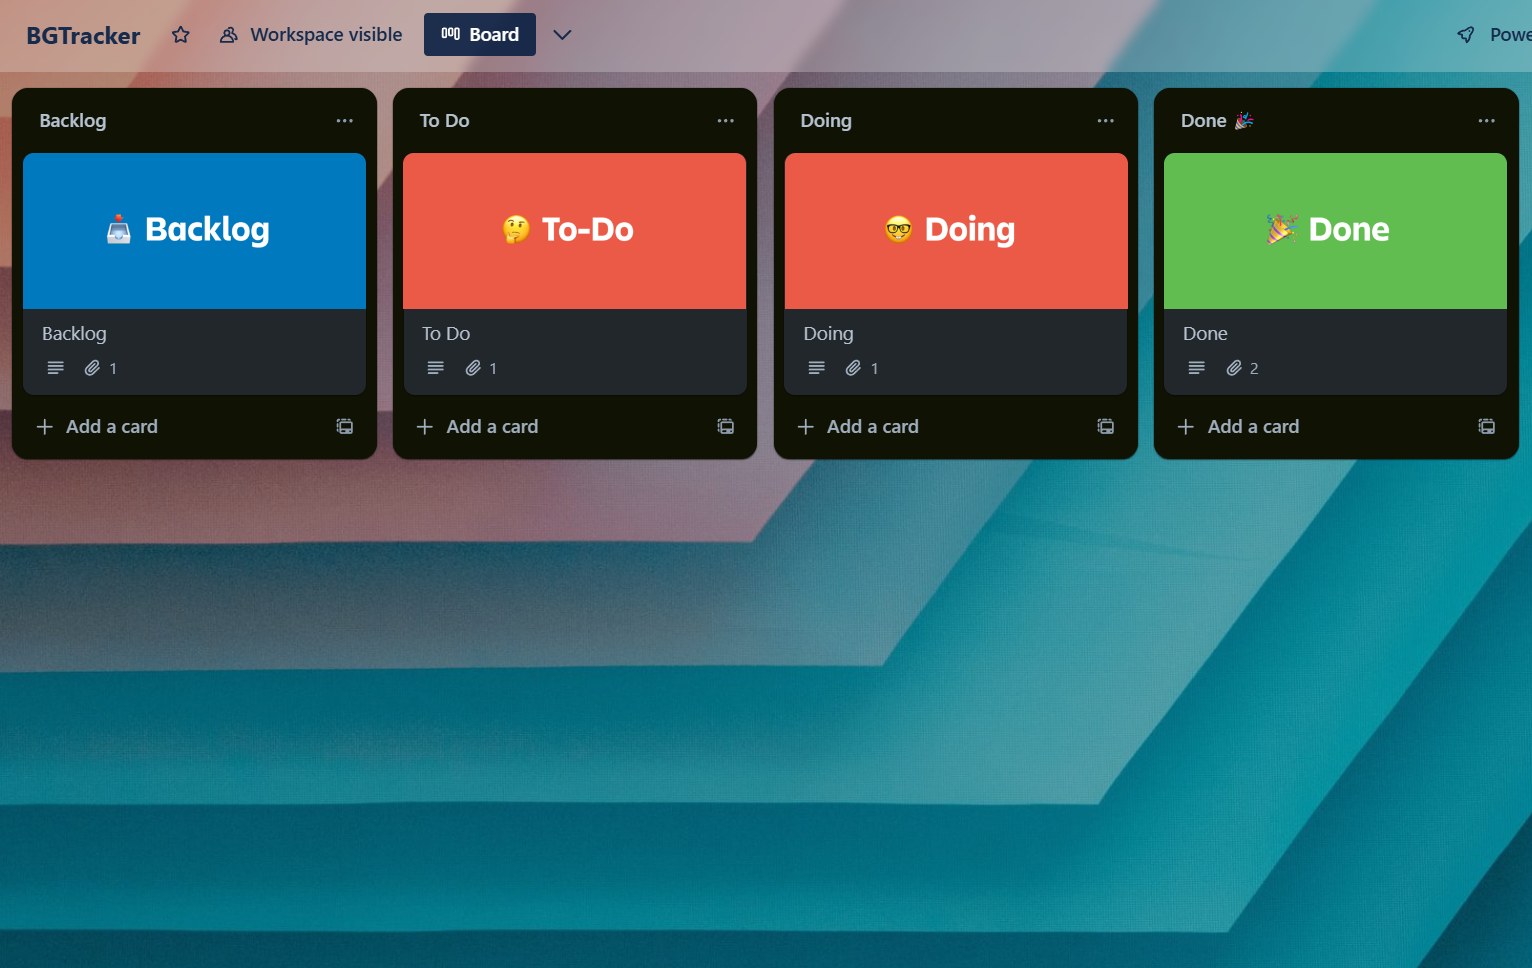
\includegraphics[width=0.9\textwidth]{media/trello1.png}
    \caption{kolumny: \textbf{Backlog}, \textbf{To do}, \textbf{Doing} oraz \textbf{Done}}
\end{figure}

\begin{figure}[H]
    \centering
    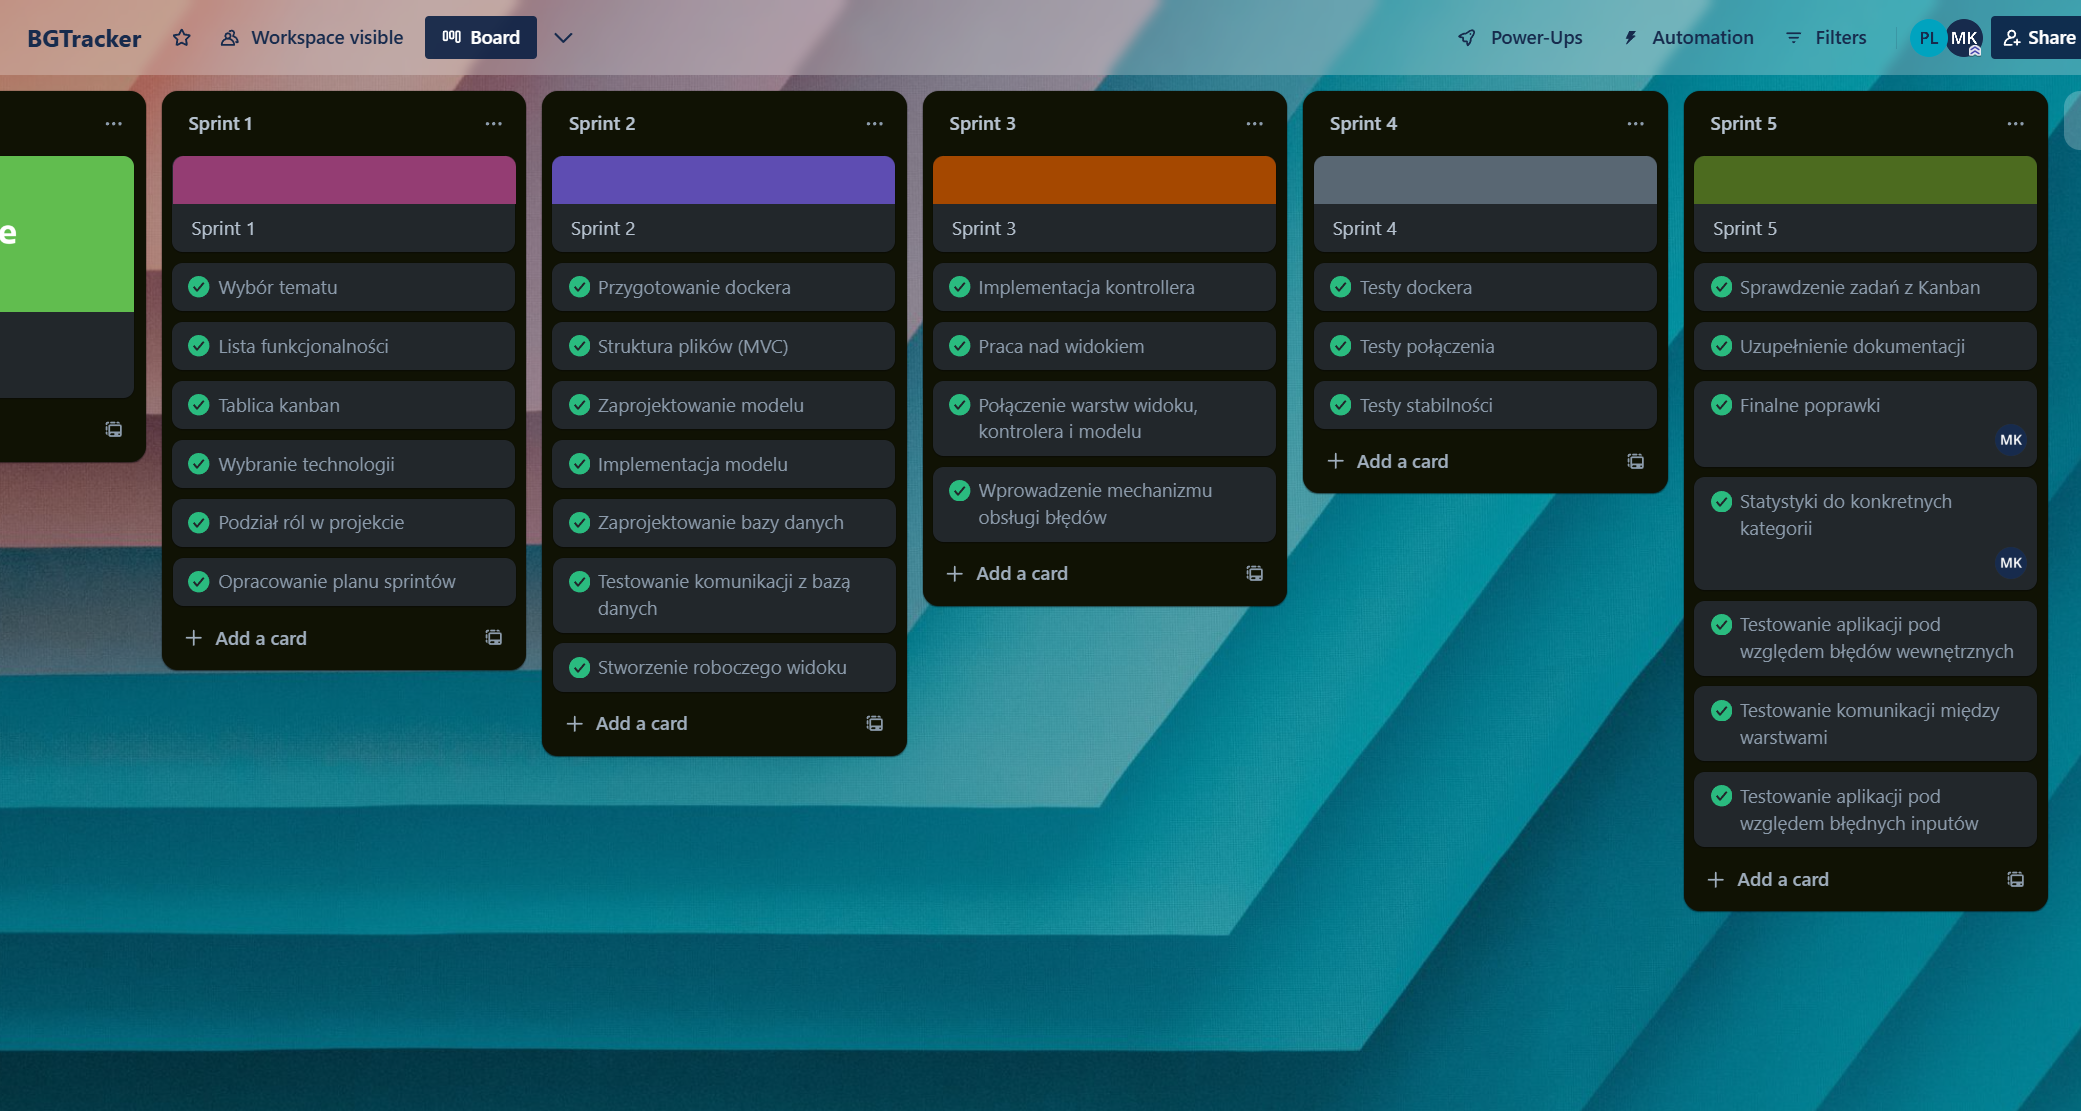
\includegraphics[width=0.9\textwidth]{media/trello2.png}
    \caption{kolumny sprintów}
\end{figure}

\pagebreak
\section{Architektura MVC}

Projekt został zaprojektowany zgodnie z wzorcem architektonicznym \textbf{Model-View-Controller (MVC)}, który pozwala na przejrzyste oddzielenie logiki biznesowej od warstwy prezentacji oraz obsługi żądań.

\begin{itemize}
    \item \textbf{Model} -- znajduje się w folderze \texttt{model} i zawiera klasy reprezentujące dane (\texttt{Game.php}, \texttt{Player.php}, \texttt{GameMatch.php}) oraz klasy obsługujące statystyki (\texttt{GameRepo.php}, \texttt{PlayerRepo.php}, \texttt{GameMatchRepo.php}) odpowiedzialne za interakcję z bazą danych.
    \item \textbf{Controller} -- folder \texttt{controller} zawiera klasy odpowiedzialne za przetwarzanie logiki aplikacji i komunikację między modelem a widokiem: \texttt{GameController.php}, \texttt{MatchController.php} \texttt{PlayerController.php}.
    \item \textbf{View} -- folder \texttt{view} przechowuje pliki \texttt{.php}, które odpowiadają za generowanie interfejsu użytkownika. Widoki są pogrupowane tematycznie w podfolderach: \texttt{game}, \texttt{match}, \texttt{player} oraz \texttt{home}.
\end{itemize}

Poniższy zrzut ekranu przedstawia strukturę katalogów w projekcie, odzwierciedlającą implementację wzorca MVC:

\begin{figure}[H]
    \centering
    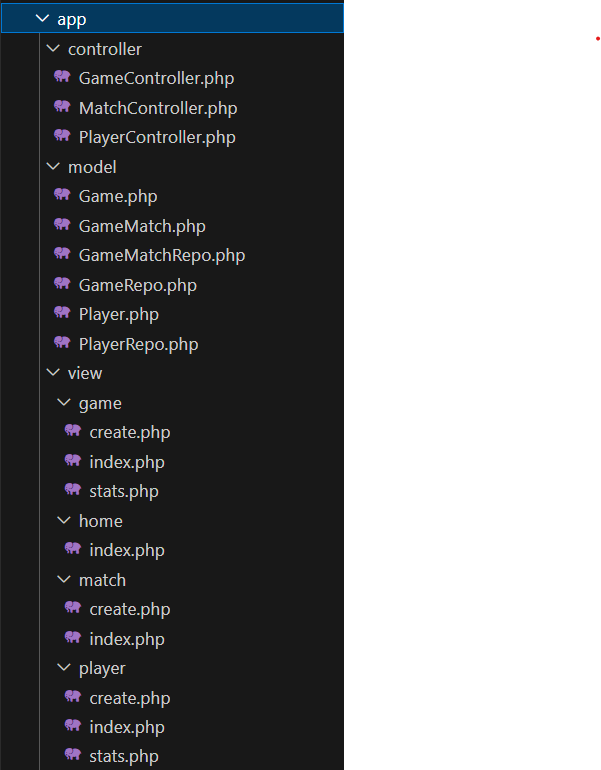
\includegraphics[width=0.5\textwidth]{media/mvc.png}
    \caption{Struktura katalogów aplikacji oparta na wzorcu MVC}
\end{figure}
\section{Schemat bazy danych}

W celu odwzorowania relacji pomiędzy encjami w naszym systemie, przygotowano diagram bazy danych w notacji UML. Baza danych została zaprojektowana w sposób umożliwiający przechowywanie informacji o grach, graczach oraz rozegranych meczach. Diagram uwzględnia kluczowe encje: \textbf{Game}, \textbf{Player}, \textbf{GameMatch} oraz tabelę pośredniczącą \textbf{MatchPlayers}, która realizuje relację wiele-do-wielu pomiędzy meczami a graczami. Diagram ten stanowi podstawę dalszego projektowania warstwy logicznej aplikacji oraz implementacji komunikacji z bazą danych.

\begin{figure}[H]
	\centering
	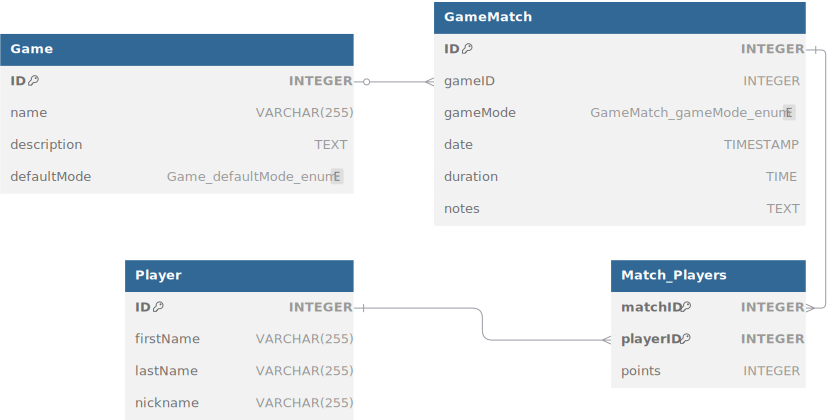
\includegraphics[width=1\linewidth]{media/baza_danych}
	\caption{Diagram bazy danych}
	\label{fig:bazadanych}
\end{figure}

\section{Ukończona aplikacja}

\subsection{Gracze}

\begin{figure}[H]
	\centering
	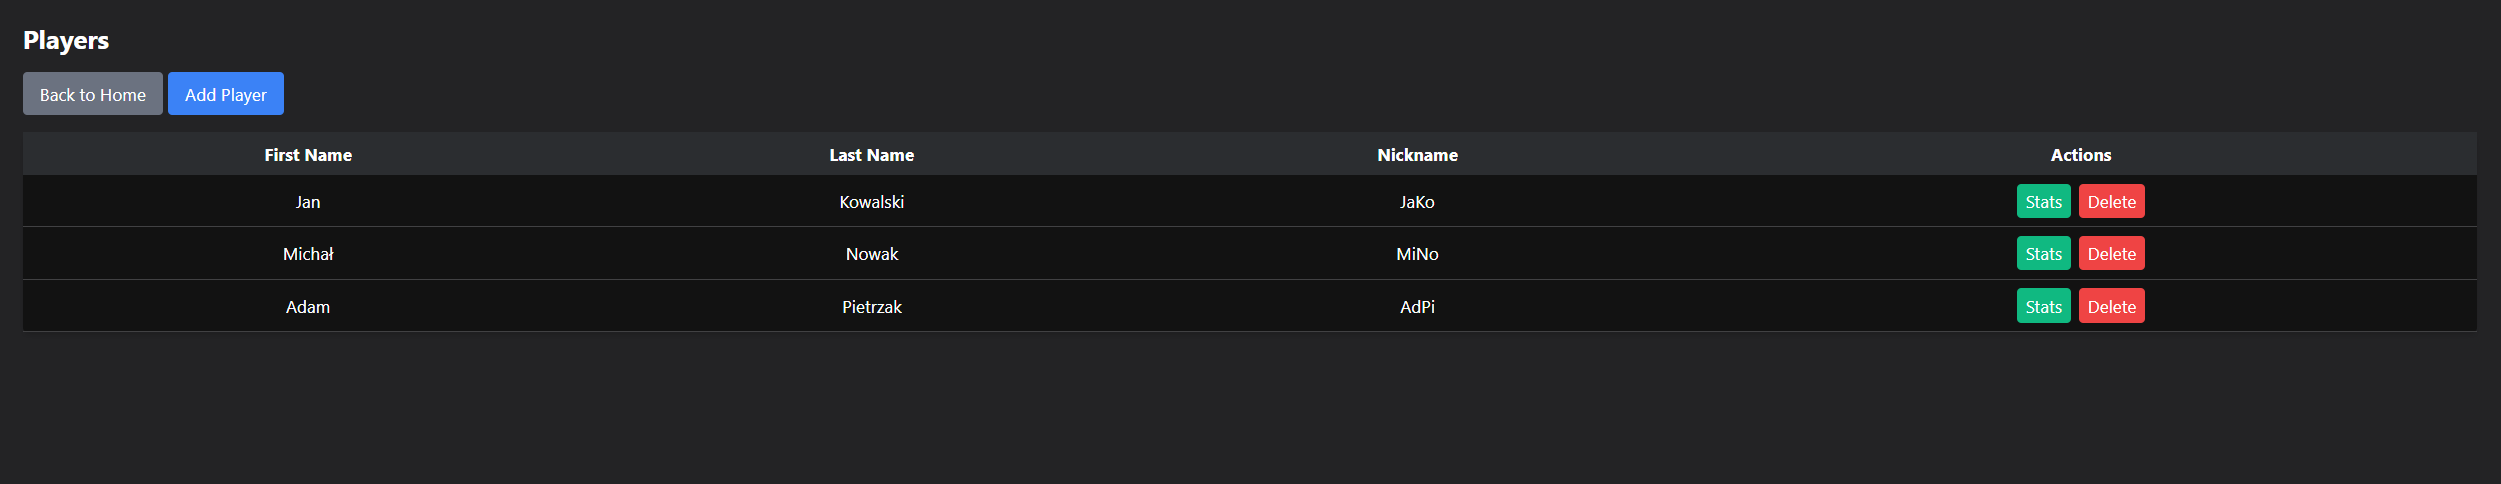
\includegraphics[width=1\linewidth]{media/1.png}
	\caption{Tabela graczy}
	\label{fig:tabelagraczy}
\end{figure}

\begin{figure}[H]
	\centering
	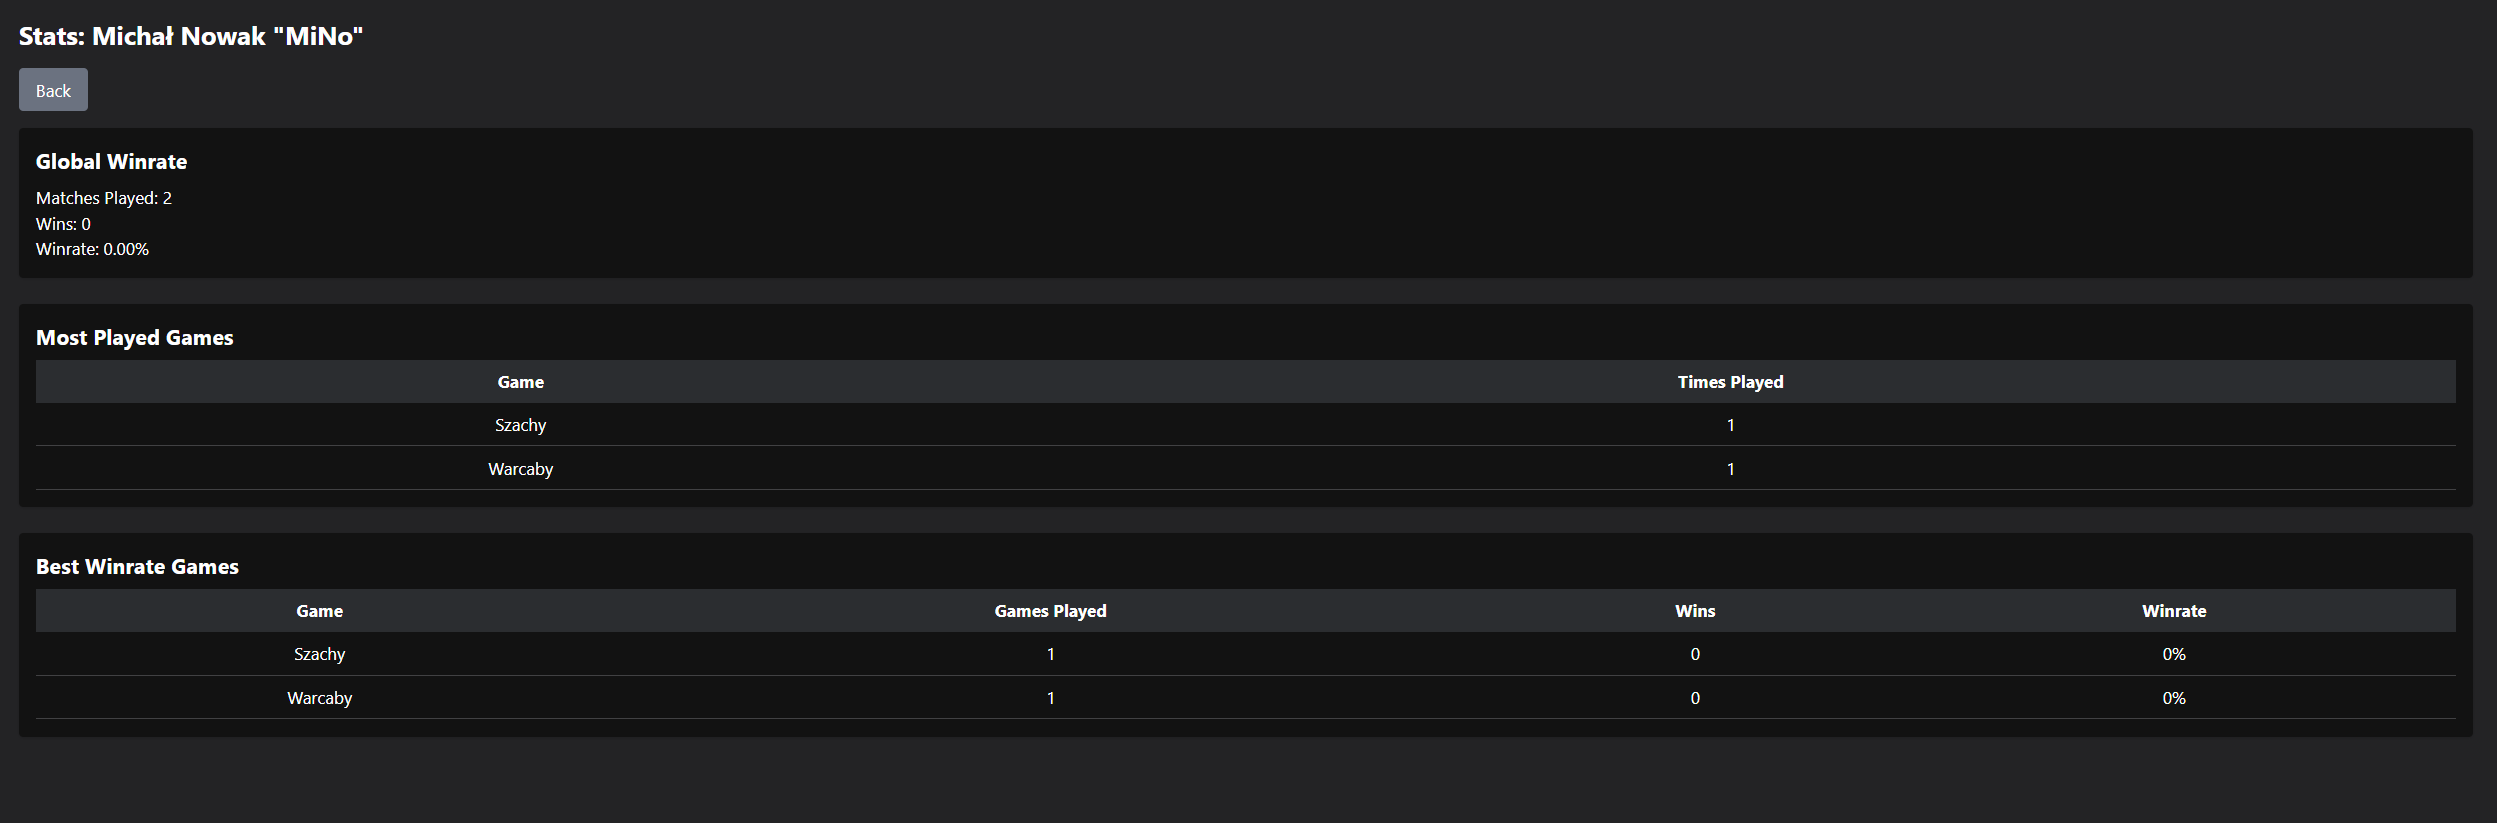
\includegraphics[width=1\linewidth]{media/4.png}
	\caption{Statystyki gracza}
	\label{fig:statystykigracza}
\end{figure}

\subsection{Gry}

\begin{figure}[H]
	\centering
	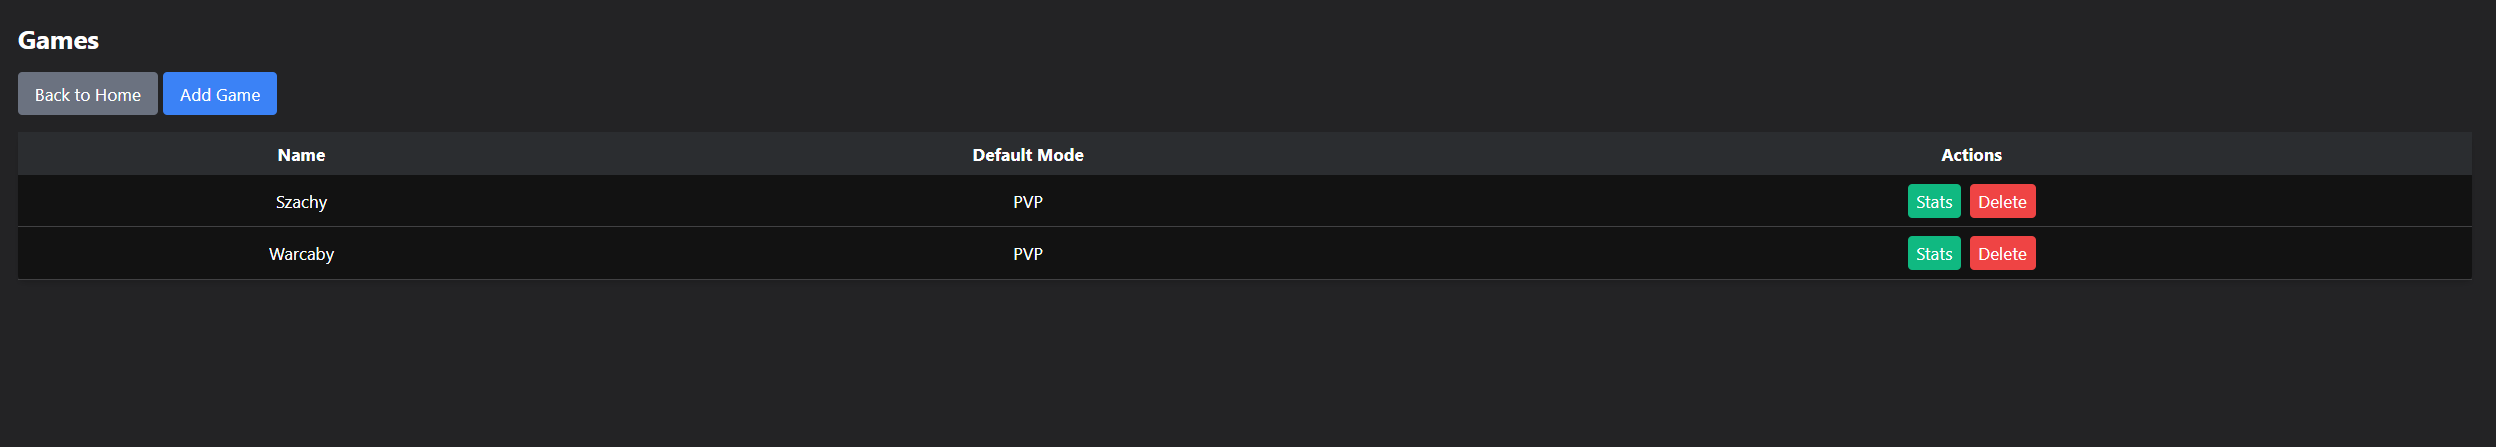
\includegraphics[width=1\linewidth]{media/2.png}
	\caption{Tabela gier}
	\label{fig:tabelagier}
\end{figure}

\begin{figure}[H]
	\centering
	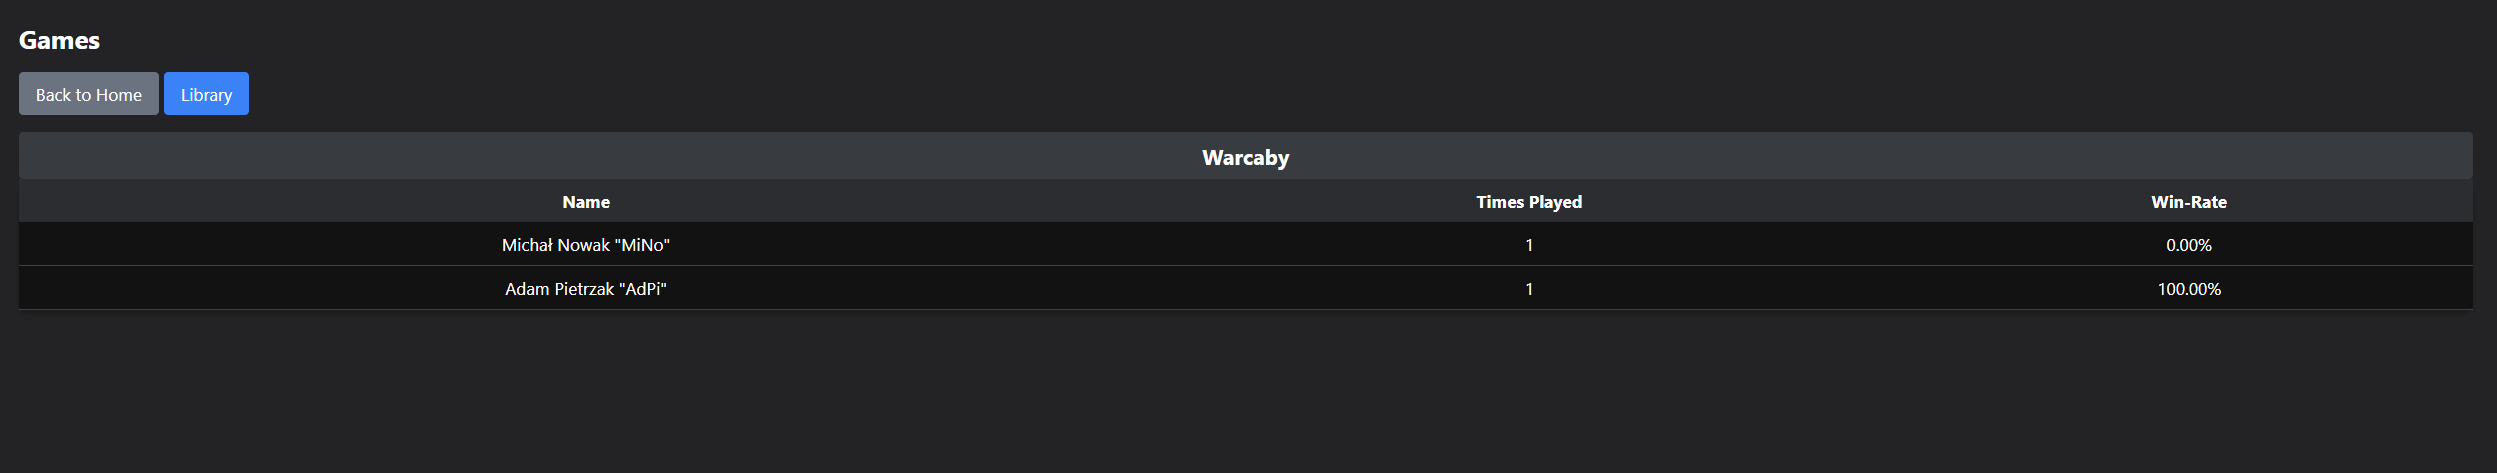
\includegraphics[width=1\linewidth]{media/5.png}
	\caption{Statystyki gry}
	\label{fig:statystykigry}
\end{figure}

\subsection{Mecze}

\begin{figure}[H]
	\centering
	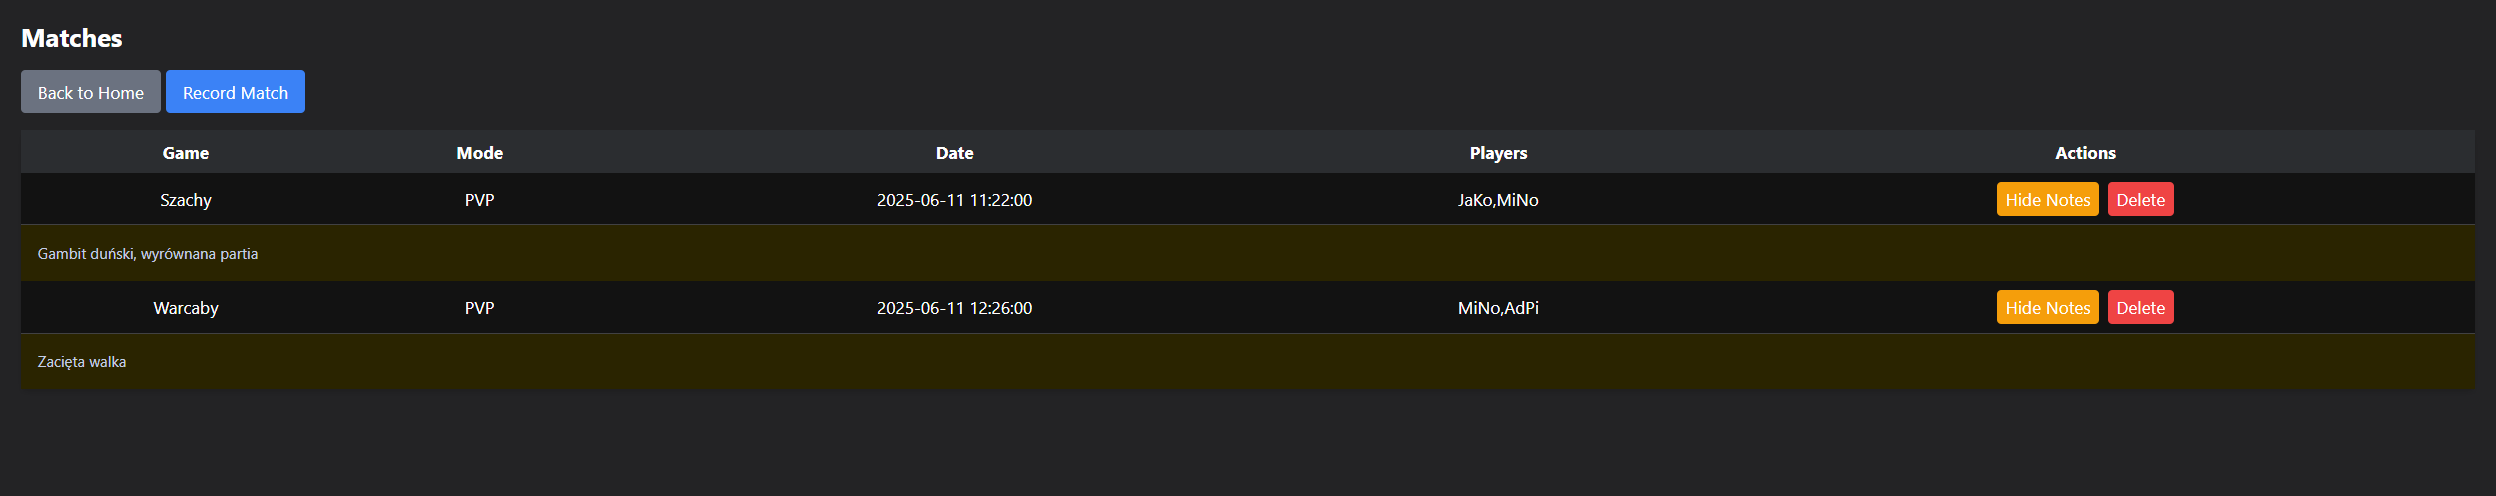
\includegraphics[width=1\linewidth]{media/3.png}
	\caption{Tabela meczy}
	\label{fig:tabelameczy}
\end{figure}

\section{Wnioski}
\begin{itemize}
	\item \textbf{Spostrzeżenia:} Praca nad aplikacją umożliwiła pogłębienie wiedzy z zakresu wzorca MVC, konteneryzacji za pomocą Dockera oraz pracy zespołowej z wykorzystaniem narzędzi takich jak Trello i GitHub. Projekt unaocznił także znaczenie jasnego podziału obowiązków oraz dobrej dokumentacji.
	\item \textbf{Osiągnięcia:} Udało się zbudować w pełni działającą aplikację webową, umożliwiającą rejestrowanie wyników gier planszowych w przejrzysty i funkcjonalny sposób. Stworzono modułowy kod z zachowaniem zasad separacji warstw, a całość została uruchomiona w środowisku Docker, co ułatwia wdrażanie i testowanie.
	\item \textbf{Potencjał rozwoju:} Projekt może być w przyszłości rozwijany o nowe funkcjonalności, takie jak: logowanie użytkowników, historia rozgrywek z filtrowaniem, generowanie statystyk i wykresów, eksport danych do plików (CSV/PDF), integracja z kontami Google lub Facebook, czy też wersja mobilna aplikacji.
\end{itemize}

\section{Bibliografia}
\begin{enumerate}
	\item Oficjalna dokumentacja PHP -- \url{https://www.php.net/docs.php}
	\item Dokumentacja Docker -- \url{https://docs.docker.com/}
	\item Dokumentacja MySQL -- \url{https://dev.mysql.com/doc/}
	\item Artykuł: „Understanding MVC Architecture" \\ -- \url{https://www.geeksforgeeks.org/mvc-design-pattern/}
	\item Oficjalna dokumentacja PDO -- \url{https://www.php.net/manual/en/book.pdo.php}
	\item Dokumentacja Git -- \url{https://git-scm.com/doc}
	\item Trello -- \url{https://trello.com}
	\item dbdiagram.io -- \url{https://dbdiagram.io}
\end{enumerate}
	
\end{document}